\documentclass{article}
\usepackage{graphicx}
\usepackage{amsmath}
\usepackage{array}
\usepackage[font=small, labelfont={sf,bf}, margin=1cm]{caption}
\usepackage{tabularx}
\usepackage{amssymb}



\date{Due: Dec 11 Edit: \today}
\title{MATH 416H HW 12}
\author{James Liu}

\begin{document}
\maketitle
\begin{itemize}
    \item [1.] Consider a set of basis \(\mathcal{ B}\) for \(V\), as it is a linear map,let \([T]_{\mathcal{BB}}=A\) be the matrix
    representation of the map, then \(p_{T}=\det(x\text{id}_V-[T]_{\mathcal{BB}})\). If expand the determinant by the first row of every sub matrix, we can see that there will be 
    a term like:\\ \((x-A_{11})(x-A_{22})(x-A_{33})\cdots\left[(x-A_{n-1,n-1})(x-A_{nn})-(A_{n-1,n}A_{n,n-1})\right]\) the highest power will be the power of multiplying every term on the main diagonal.
    And as \(A\) is a \(n\times n\) matrix, there will be n terms on the main diagonal which means that the degree is n.
    \item [2.]
    \begin{itemize}
        \item [a)] By definition, \(S(w)=T_W(w)\), then \(S\circ S(w)=T_W\circ T_W(w)\) which is equivalent to \([S]^2w=[T]_W^2w\) and
        similarly \([S]^kw=[T]_W^kw\) therefore:
        \begin{align*}
            p(S)&=a_1\text{id}_W+a_2S+a_3S^2+\cdots\\
            &=a_1\text{id}_W+a_2T|_W+a_3T|_W^2+\cdots\\
            &=p(T)|_W
        \end{align*}
        \item [b)] Note the minimal polynomial of \(T\) as \(m_T\).
        \begin{align*}
            m_T&=a_0x^0+a_1x^1+\cdots+a_nx^n\\
            m_T(S)&=a_0\text{id}_W+a_1S^1+\cdots+a_nS^n\\
            &=a_0\text{id}_W+a_1T|_W^1+\cdots+a_nT|_W^n=m_T(T|_W)\\
            \text{as } m_T(T)=0\\
            m_T(T|_W)w&=m_T(S)w=0, \ \forall w\in W
        \end{align*}
        Since \(m_{S}(x)\) is the minimal polynomial of \(S\), it divides any polynomial that annihilates \(S\).
    \end{itemize}
    \item [3.]
    \begin{itemize}
        \item [a)]
        \begin{align*}
            p_T(x)&=\det(x\ \text{id}-A)\\
            &=\left|\begin{matrix}
                x-2&-1&0&1\\
                0&x-3&-1&0\\
                0&1&x-1&0\\
                0&-1&0&x-3
            \end{matrix}\right|\\
            &=(x-2)(x-3)[(x-3)(x-1)-(-1)\times 1]\\
            &=(x-2)(x-3)[x^2-4x+4]\\
            &=(x-2)^3(x-3)
        \end{align*}
        \item [b)]
        \begin{align*}
            \det(A-x\ \text{id})&=0\\
            (x-2)^3(x-3)&=0\\
            \lambda_1=2&\quad\lambda_2=3\\
            (A-2)v&=\begin{pmatrix}
                0&-1&0&1\\
                0&1&-1&0\\
                0&1&-1&0\\
                0&-1&0&1
            \end{pmatrix}v=0\\
            v&=\begin{bmatrix}
                s\\k\\k\\k
            \end{bmatrix}\\
            (A-3)v&=\begin{pmatrix}
                -1&-1&0&1\\
                0&0&-1&0\\
                0&1&-2&0\\
                0&-1&0&0
            \end{pmatrix}v=0\\
            v&=\begin{bmatrix}
                s\\0\\0\\s
            \end{bmatrix}
        \end{align*}
        Therefore , there are 3 distinct eigenvectors:
        \begin{align*}
            \lambda&=2\\
            v_1=\begin{pmatrix}
                1\\0\\0\\0
            \end{pmatrix}
            &\quad v_2=\begin{pmatrix}
                0\\1\\1\\1
            \end{pmatrix}\\
            \lambda&=3\\
            v_3&=\begin{pmatrix}
                1\\0\\0\\1
            \end{pmatrix}
        \end{align*}
        \(\forall v\in E_\lambda\), \(v\) is either linear combination of \(v_1\) and \(v_2\) or a complex multiply of \(v_3\)
        \item [c)]
        A is not diagonalizable as the number of distinct eigenvectors does not equal to 4.
    \end{itemize}
    \item [4.]
    \begin{itemize}
        \item [a)]
        \begin{align*}
            \det(A-x\ \text{id})&=0\\
            \left|\begin{matrix}
                -1-x&3&0\\
                0&2-x&0\\
                2&1&-1-x
            \end{matrix}\right|&=0\\
            v&=(-1-x)(-1-x)(2-x)\\
            \lambda_1=-1,&\quad \lambda_2=2\\
            (A+1\ \text{id})v&=0\\
            \left(\begin{matrix}
                0&3&0\\
                0&3&0\\
                2&1&0
            \end{matrix}\right)v&=0\\
            %
            (A-2\ \text{id})v&=0\\
            v&=\begin{pmatrix}
                0\\0\\s
            \end{pmatrix}\\
            \left(\begin{matrix}
                -3&3&0\\
                0&0&0\\
                2&1&-3
            \end{matrix}\right)v&=0\\
            v&=\begin{pmatrix}
                s\\s\\s
            \end{pmatrix}\\
            J_A&=\begin{bmatrix}
                -1&1&0\\
                0&-1&0\\
                0&0&2
            \end{bmatrix}
        \end{align*}
        \item [b)]
        \begin{align*}
            \lambda&=-1\\
            v_1&=(0,0,1)^T\\
            \lambda&=2\\
            v_3&=(1,1,1)^T
        \end{align*}
        As for \(\lambda=-1\), the geometrix multiplicity is 1 and algebratic is 2:
        \begin{align*}
            Av_2&=\lambda_1v_2+v_1\\
            (A+1)v_2&=v_1\\
            \begin{bmatrix}
                0&3&0\\
                0&3&0\\
                2&1&0
            \end{bmatrix}v_2&=\begin{bmatrix}
                0\\0\\1
            \end{bmatrix}\\
            v_2&=\begin{bmatrix}
                \frac{1}{2}\\0\\0
            \end{bmatrix}\\
            K&=\begin{bmatrix}
                0&0.5&1\\
                0&0&1\\
                1&0&1
            \end{bmatrix}\\
            K^{-1}&=\begin{bmatrix}
                0&-1&1\\
                2&-2&0\\
                0&1&0
            \end{bmatrix}\\
            A&=KJK^{-1}\\
            J&=K^{-1}AK\\
            K&=S^{-1}\\
            K^{-1}&=S
        \end{align*}
    \end{itemize}
    \item [5.]
    \begin{align*}
        \begin{bmatrix}
            7&1&0&0&0&0&0\\
            0&7&0&0&0&0&0\\
            0&0&7&1&0&0&0\\
            0&0&0&7&0&0&0\\
            0&0&0&0&3&0&0\\
            0&0&0&0&0&3&1\\
            0&0&0&0&0&0&3\\
        \end{bmatrix}
    \end{align*}
    As the minimal polynomial indicates that the for 7, the algebratic multiplicity is 4 and the largest jordan block size is 2 similar for 3, the algebratic multiplicity is 3 whith largest jordan block size being 2.
    \item [6.]
        \begin{align*}
            S(A)&=\lambda A\\
            A^T&=\lambda A\\
           S(A^T)&=S(\lambda A)\\
           A&=\lambda \times A^T\\
           &=\lambda^2 A\\
           \lambda &=\pm1
        \end{align*}
        Consider when \(\lambda =1\)
        \begin{align*}
            A^T&=A\\
            \text{note such matrix as:} X
        \end{align*}\\
        When \(\lambda =-1\)
        \begin{align*}
            A^T&=-A\\
            \text{note such matrix as:} Y
        \end{align*}
        \begin{align*}
            A&=\frac{1}{2}(A+A^T)+\frac{1}{2}(A-A^T)\\
            \frac{1}{2}(A+A^T)^T&=\frac{1}{2}(A^T+A)=X\\
            \frac{1}{2}(A-A^T)^T&=-\frac{1}{2}(A-A^T)=Y\\
            A&=\frac{1}{2}X+\frac{1}{2}Y
        \end{align*}
        Which means that \(S(A)\) do have a eigen basis which means that it is diagonalizable.
    \item [7.]
    \begin{itemize}
        \item [a)]\
        \begin{itemize}
            \item [exists a zero vector:] For \(M=[0]_n\)(n\(\times\)n zero matrix), \(\forall A\in\mathcal{H}_n\), \(A+M=A\)
            \item [addition:] \(\forall A\in \mathcal{H}_n,\mu \in \mathbb{R}\)
                \begin{align*}
                    (A+B)_{ij}&= A_{ij}+B_{ij}\\
                    &=\overline{A}_{ji}+\overline{B}_{ji}\\
                    &=(A+B)^*_{ij}
                \end{align*}
            \item [multiplication:]
            \begin{align*}
                \lambda A_{ij}&=\lambda A_{ij}\\
                (\lambda A_{ij})^*&=\lambda (A_{ij})^*
            \end{align*}
        \end{itemize}
        And it also follows the rest axioms about algebra which makes it a vector space over \(\mathbb{R}\).\\
        However, scaler multiplication is no longer close under \(\mathbb{C}\) thus it is not a vector space over\(\mathbb{C}\)
        \item [b)]
        the dimention will be \(\dim(\mathcal{H}_n)=n+2\times ((n-1)+(n-2)+\cdots+1)=n^2\),
        \(\mathcal{B}=\{b_1,b_2,\cdots,b_n^2\}\). The basis would be:
        \begin{figure}[h]
            \centering
            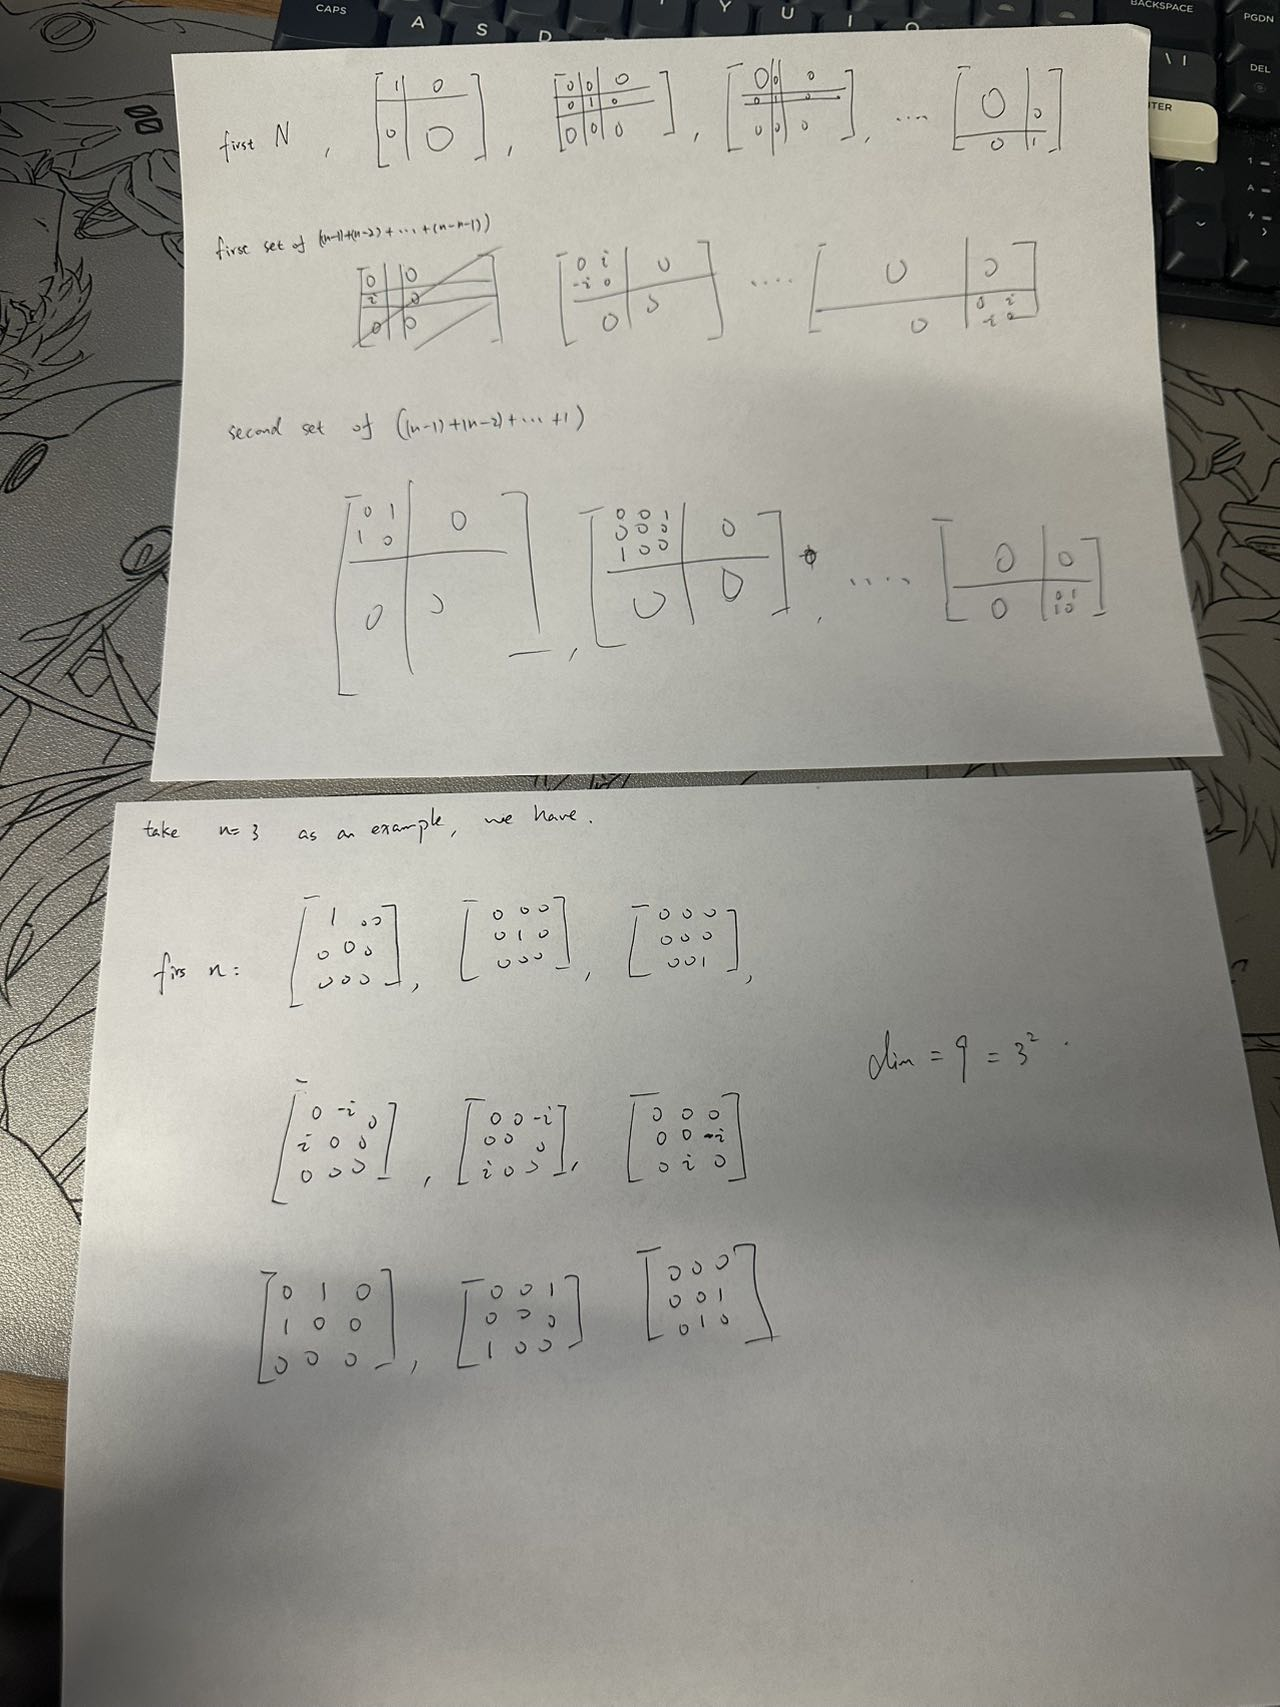
\includegraphics[scale=0.2]{math416_hw12.jpeg}
        \end{figure}
    \end{itemize}
    \newpage
    \item [8.]
    \(\mathcal{B}=\{E_{11},E_{12},E_{21},E_{22}\}\). Then, we have:
    \begin{align*}
        T&=\begin{pmatrix}
            3&0&0&0\\
            0&2&1&0\\
            0&1&2&0\\
            0&0&0&3
        \end{pmatrix}\\
        \det(T-x\text{ id}_4)&=0\\
        \left|\begin{matrix}
            3-x&0&0&0\\
            0&2-x&1&0\\
            0&1&2-x&0\\
            0&0&0&3-x
        \end{matrix}\right|&=0\\
        (3-x)^2[(2-x)^2-1]&=0\\
        (3-x)^3(1-x)&=0\\
        \lambda_1=3&\ \lambda_2=1
    \end{align*}
    find eigenvectors:\\
    \begin{align*}
        \lambda_1&=3\\
        (T-3\text{ id}_4)v&=0\\
        v&=(s,k,k,t)\\
        \lambda_2&=1\\
        (T-1\text{ id}_4)v&=0\\
        v&=(0,s,-s,0)
    \end{align*}
    Therefore it does have a eigenbasis, which gives:
    \begin{align*}
        J&=\begin{bmatrix}
            3&0&0&0\\
            0&3&0&0\\
            0&0&3&0\\
            0&0&0&1
        \end{bmatrix}\\
        b_1&=(1,0,0,0)=\begin{pmatrix}
            1&0\\0&0
        \end{pmatrix}\\
        b_2&=(0,1,1,0)=\begin{pmatrix}
            0&1\\1&0
        \end{pmatrix}\\
        b_3&=(0,0,0,1)=\begin{pmatrix}
            0&0\\
            0&1
        \end{pmatrix}\\
        b_4&=(0,1,-1,0)=\begin{pmatrix}
            0&1\\
            -1&0
        \end{pmatrix}
    \end{align*}
\end{itemize}
\end{document}